%!TeX root = ../numapde-OptiPuls-2.tex
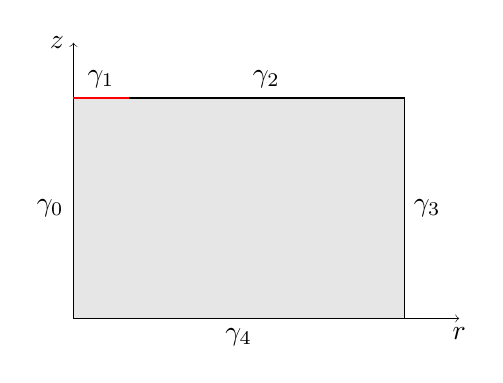
\begin{tikzpicture}[scale=0.7]
	% axes
	\draw [->, very thin] (0, 0) -- (7, 0) node[below] {$r$};
	\draw [->, very thin] (0, 0) -- (0, 5) node[left] {$z$};

	% rectangle
	\draw [fill=gray, fill opacity=0.2] (0, 0) -- (6, 0) -- (6, 4) -- (0, 4) -- cycle;

	% labels
	\node[left] at (0, 2) {$\gamma_0$};
	\node[above] at (0.5, 4) {$\gamma_1$};
	\node[above] at (3.5, 4) {$\gamma_2$};
	\node[right] at (6, 2) {$\gamma_3$};
	\node[below] at (3, 0) {$\gamma_4$};

	\draw [red] (0, 4) -- (1, 4);
\end{tikzpicture}
